\documentclass{beamer}
\usetheme{Boadilla}
\usepackage[polish]{babel}
\usepackage[utf8]{inputenc}
\usepackage[T1]{fontenc}
\usepackage{listings}
\usepackage[makeroom]{cancel}

\begin{document}
\title{Chaos Deterministyczny} 
\author{Przemysław Czechowski} 
\date{\today} 

\frame{\titlepage} 

\begin{frame}[fragile]
Problem dwóch ciał?\pause
\begin{lstlisting}
play.py two_bodies
\end{lstlisting}
\end{frame}

\begin{frame}[fragile]
Problem trzech ciał?
\begin{lstlisting}
play.py threeA
play.py threeB
play.py threeC
\end{lstlisting}
\end{frame}

\begin{frame}{Stabilność układu słonecznego}\pause
\begin{itemize}
\item Czy ziemia zostanie wystrzelona?\pause
\item Czy ziemia może zderzyć się z inną planetą?\pause
\item Jeśli tak, to kiedy?\pause
\end{itemize} 

1887 - nagroda Króla Szwecji: rozwiązać problem N ciał oddziałujących grawitacyjnie\pause\\
Henri Poincaré zdobywa nagrodę, chociaż nie rozwiązał problemu\pause
\end{frame}

\begin{frame}{Chaos (wg. Royal Society, 1987)}
\pause
\textbf{ Stochastyczne zachowanie występujące w układzie daterministycznym}\pause

Przykłady:\pause
\begin{itemize}[<+->]
\item Problem >2 ciał
\item Przewidywanie pogody
\item Wzrost niestabilny
\item Przepływ turbulentny
	\begin{itemize}[<+->]
		\item Palce lepkości
		\item Wzrost sieci rzecznej
		\item Spalanie papieru w wąskiej szczelinie
	\end{itemize} 
\end{itemize} 
\end{frame}

\begin{frame}{Palce lepkości} \pause
\centering
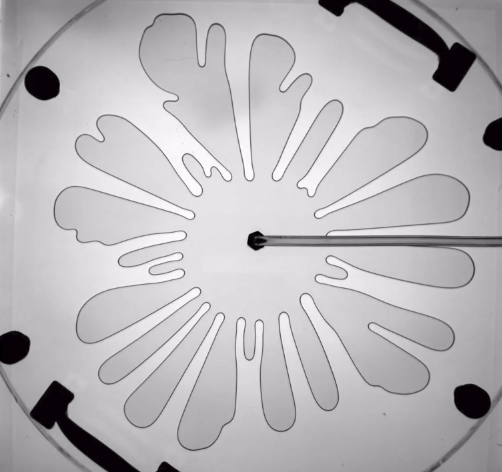
\includegraphics[height=0.6\textheight]{viscous_fingers}
\url{https://www.youtube.com/watch?v=BgeKR9HuY9s}

\end{frame}

\begin{frame}[fragile]
\textbf{ Stochastyczne zachowanie występujące w układzie daterministycznym}
\begin{lstlisting}
play.py butterfly
\end{lstlisting}
\end{frame}

\begin{frame}[t]{Wykładniki Lyapunowa - teoria}
\begin{equation*}
| \delta\mathbf{x}(t) | \approx e^{\lambda t} | \delta \mathbf{x}(0) |
\end{equation*}
\end{frame}

\begin{frame}[t]{Wykładniki Lyapunowa - praktyka}
\begin{equation*}
| \delta\mathbf{x}(t) | \approx e^{\lambda t} | \delta \mathbf{x}(0) |
\end{equation*}
\centering
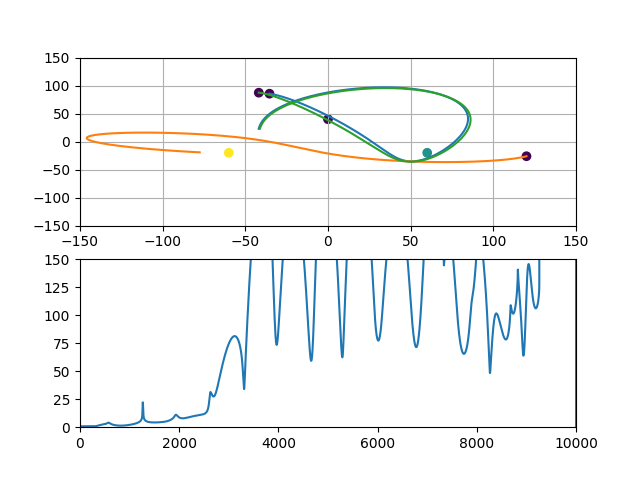
\includegraphics[height=0.7\textheight]{lyapunov}
\end{frame}

\begin{frame}[t]{Wykładniki Lyapunowa - praktyka}
\begin{equation*}
| \delta\mathbf{x}(t) | \approx e^{\lambda t} | \delta \mathbf{x}(0) |
\end{equation*}
\centering
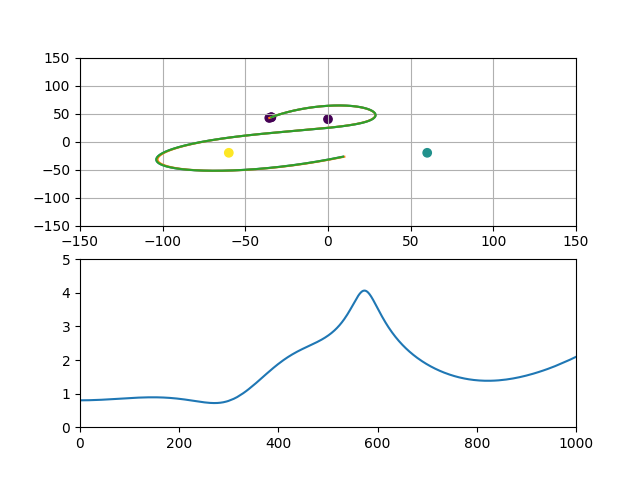
\includegraphics[height=0.7\textheight]{lyapunov_short}
\end{frame}

\begin{frame}[t]{Wykładniki Lyapunowa - praktyka}
\begin{equation*}
| \delta\mathbf{x}(t) | \approx e^{\lambda t} | \delta \mathbf{x}(0) |
\end{equation*}
\centering
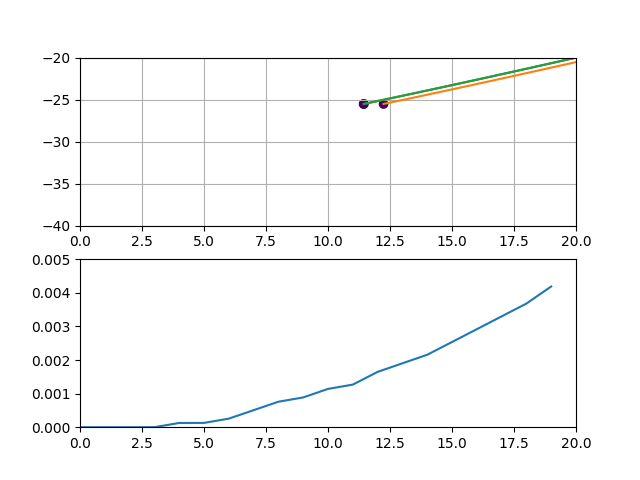
\includegraphics[height=0.7\textheight]{lyapunov_very_short}
\end{frame}

\begin{frame}{Alternatywa dla wykładników Lyapunowa} \pause
\begin{itemize}
	\item Etropia metryczna
	\item Etropia topologiczna
\end{itemize} 
Wymagają innego opisu
\end{frame}

\begin{frame}{Przepływ zamiast równań} \pause
\centering
\begin{equation*}
\xcancel{\dot{x}=y, \dot{y}=\sin{x}}
\end{equation*}
\begin{equation*}
\downarrow
\end{equation*}
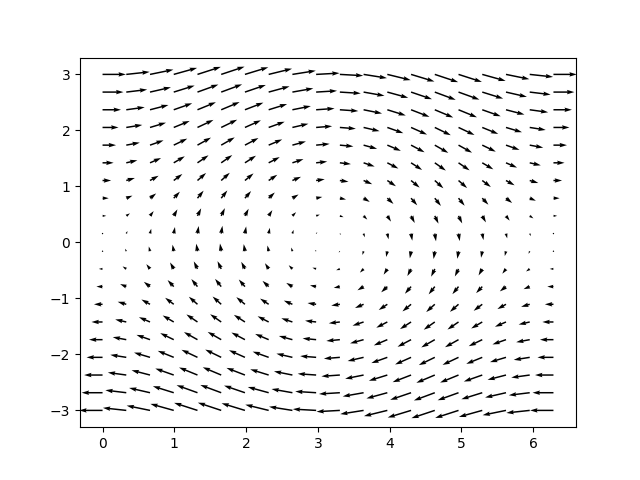
\includegraphics[height=0.7\textheight]{phase_portrait}
\end{frame}

\begin{frame}{Przekroje Poincaré} \pause
Przepływ w N wymiarach $\leftarrow$ Mapa w N-1 wymiarach\\ \pause
Kiedy trajektoria znowu przejdzie przez powierzchnię?\\ \pause
\end{frame}

\begin{frame}{Przekroje Poincaré - przykład}
\centering
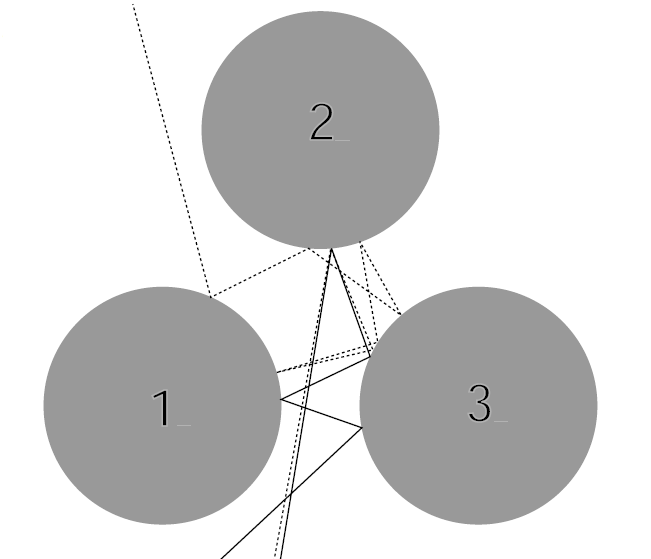
\includegraphics[height=0.7\textheight]{pinball}\\
Każde zderzenie charakteryzuje pozycja i kąt - dwa stopnie swobody\\
Mapa - od jednego zderzenia do kolejnego
\end{frame}

\begin{frame}{Przekroje Poincaré - przykład}
\centering
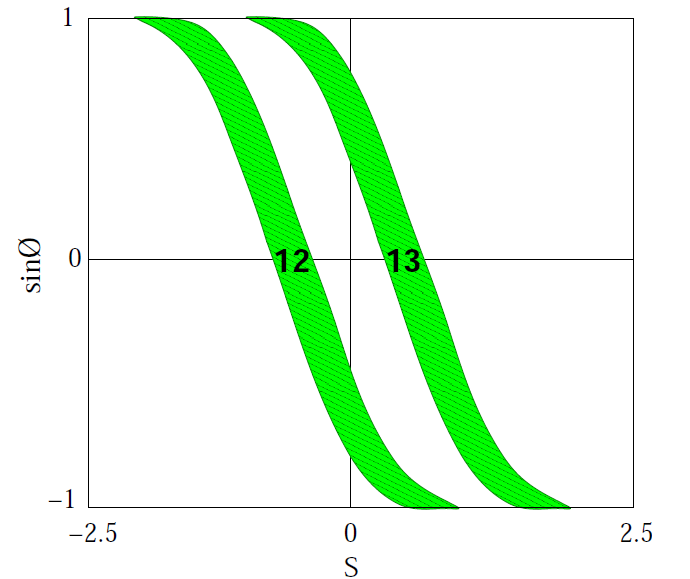
\includegraphics[height=0.7\textheight]{poincare_section}\\
Cały kwadrat mapuje się na zielony obszar w pierwszej iteracji (mapa nieodwracalna)
\end{frame}

\begin{frame}{Entropia metryczna} \pause
	Załóżmy, że mamy odwracalną mapę $M$ na zbiorze $S$.\pause \\
	Chcemy opisać ,,chaotyczność`` $M$ - jak bardzo miesza $S$.\\ \pause
	Zbiór $W$ dzielimy na trzy podzbiory: $\{W_1, W_2, W_3\} = \{W_i\}$.\pause
	Wiemy, że w kolejnych $n$ iteracjach mapy punkt $x_0$ trafiał do zbiorów
  $W_{i_1}, W_{i_2}, \dots W_{i_n}$\pause\\
	Co możemy powiedzieć o warunku początkowym $x_0$?\pause
	\begin{equation*}
		x_0 \in W_{i_1} \cap M^{-1}(W_{i_2}) \cap \dots \cap M^{-n+1}(W_{i_n})
	\end{equation*}
\end{frame}

\begin{frame}{Entropia metryczna, cd.}
	\begin{equation*}
		x_0 \in W_{i_1} \cap M^{-1}(W_{i_2}) \cap \dots \cap M^{-n+1}(W_{i_n})
	\end{equation*}
	Jak wiele informacji daje nam ,,symboliczna`` trajektoria $i_1 \dots i_n$?\\ \pause
	$\{W^{(n)}_i\}$ - rodzina $n^3$ zbiorów postaci
	$W_{i_1} \cap M^{-1}(W_{i_2}) \cap \dots \cap M^{-n+1}(W_{i_n})$ \pause \\
	Informacja Shannona:
	\begin{equation*}
		H(\mu, \{W^{(n)}_i\})=\sum_{W \in \{W^{(n)}\}}\mu(W)\ln\frac{1}{\mu(W)}
	\end{equation*}
	$\mu$ - miara probabilistyczna\\ \pause
	Entropia metryczna:
	\begin{equation*}
		h(\mu, M) = \sup_{\{W_i\}}\lim_{n\to\infty}\frac{1}{n}H(\mu, \{W_i^{(n)}\})
	\end{equation*}
\end{frame}

\begin{frame}{Entropia metryczna, cd2.}
	Entropia metryczna:
	\begin{equation*}
		h(\mu, M) = \sup_{\{W_i\}}\lim_{n\to\infty}\frac{1}{n}H(\mu, \{W_i^{(n)}\})
	\end{equation*}
	Fakt: 
	\begin{equation*}
		H(\mu, \{W^{(n)}_i\}) - H(\mu, \{W^{(n)}_i\}) = h(\mu)
	\end{equation*}
 $h(\mu)$ to informacja o $x_0$ jaką dostajemy z każdą kolejną iteracją
\end{frame}

%\begin{frame}{Entropia topologiczna}
%	Zamiast miary - liczenie zbiorów
%	\begin{equation*}
%		h_T(M) = \sup_{\{W_i\}}\lim_{n\to\infty}\frac{1}{n}|{W_i^{(n)}\}|)
%	\end{equation*}
%	\begin{itemize}
%		\item $h_\mu, h_T > 0 $ dla układów chaotycznych i zerowe dla niechaotycznych
%		\item Trudne do obliczenia dla rzeczywistych układów
%	\end{itemize} 
%\end{frame}

\begin{frame}{Epilog - stabilność układu słonecznego}
	\begin{equation*}
	| \delta\mathbf{x}(t) | \approx e^{\lambda t} | \delta \mathbf{x}(0) |
	\end{equation*}
	\pause
	Dla układu słonecznego $\lambda \approx 1/1\ \Myr$ \cite(laskar1989numerical)
\end{frame}

\begin{frame}
\nocite{stewart1994czy}
\nocite{ott2002chaos}
\nocite{ChaosBook}
\bibliography{mybib}{}
\bibliographystyle{plain}
\end{frame}

\end{document}
